\chapter{Visual servoing} 
\label{Chap:Visual-Servoing}


\section{Visual servoing and MPC}

\label{sec:vs}

Visual servoing aims at controlling the motion of a robot equipped with a camera, by minimizing errors between observed features and their corresponding reference features. The nature of the features differentiates schemes of visual servoing: Image based visual servoing (IBVS) uses only image features; Position based visual servoing (PBVS) uses the 3-D pose(s) of object(s) of interest. In any of these cases of feedback, one may use a velocity controller such as

$$
\text{v}^c = -\lambda L_e^{+}e,
$$

where $e$ is the vector of errors, $\text{v}^c$ is the velocity of the camera and $L_e^{+}$ is the Moore-Penrose pseudo-inverse of the interaction matrix $L_e$, that is, the matrix relating the velocity of the features and the velocity of the camera.

Now, in walking pattern generation (see Section~\ref{sec:wpg}), MPC is used to estimate a sequence of optimal controls at some horizon, because of the step-based nature of walking. Hence, we want to orient the optimization of the foot placement by taking into account the expected evolution of the visual servoing (VS) errors so that, instead of minimizing the VS errors at current time $k$, one would like to foresee its evolution at some horizon $[k+1,k+N]$. 

In~\cite{Allibert2010}, such a time horizon-aware scheme has been proposed. The visual predictive control (VPC) is introduced as:

\begin{eqnarray}
\label{Eq:MinVisualFeatures}
 \min_{U_{k}} \;&& \sum\limits_{j=k+1}^{k+N} [s^d_j - s^m_j]^{\transpose} W_j [s^d_j - s^m_j], \\
 \mbox{subject to} \; && s^d_j = s^{*}_j - \epsilon_j, \\
 \label{Eq:ConstraintDynamicModel}
 && q_j = f(q_{j-1},u_{j-1}), \\
 \label{Eq:ConstraintProjection}
 && s^m_j = h(q_j).
\end{eqnarray}

In Eq.~\ref{Eq:MinVisualFeatures}, $U_{k}=u_{k:k+N-1}$ are the series of controls to be applied, $q_j$ is the state, and $s^*_j$, $s^d_j$ and $s^m_j$ are respectively the reference, desired and predicted positions of the visual features. The terms $\epsilon_j$ are the errors $s_j-s^m_j$ between real and predicted feature positions.
Allibert et al. assume $\epsilon_j$ constant over the prediction horizon, equal to $\epsilon_k=s_k-s^m_k$, i. e. the error at current time $k$, because by definition the $s_j$ are not known for $j>k$.
Since our landmarks are static, $s^*_j \stackrel{\mbox{\tiny def}}{=} s^*$, and since the prediction errors are constant on the horizon window, $s^d_j=s^d_k=s^*-\epsilon_k$ are constant in the prediction horizon.

Eq.~\ref{Eq:ConstraintDynamicModel} is the dynamic model, that estimates the new state given the last state/control pair. In general, this function is non-linear. We will see how to deal with this non-linearity.

Eq.~\ref{Eq:ConstraintProjection} is also a non-linear function that estimates the output of the model $s^m_j$, given the current state $q_j$. This equation implements the pinhole camera projection model.

Matrix $W_j$ in Eq.~\ref{Eq:MinVisualFeatures} is a positive definite matrix  used to weight errors in the prediction horizon. As suggested in~\cite{Allibert2010}, we   consider equal weights for all features errors, $W_j = diag(w_j)$. 

Here, $s^m_j$ is the collection of all the predicted features at time $j$, that is, for $M$ features $s^m_j = ( s_{1,j}^m, s_{2,j}^m, \hdots, s_{M,j}^m )^{\transpose} $. Eq.~\ref{Eq:MinVisualFeatures} can be rewritten as

\begin{equation}
\label{Eq:MinVisualFeatures2}
 \min_{U_{k}} \; \sum\limits_{l=0}^{M}  [S^d_{l} - S^m_{l,k}]^{\transpose} W [S^d_{l} - S^m_{l,k}],
\end{equation}

with $S^m_{l,k}$ stacking the features positions in the horizon: $S^m_{l,k} =  \left(
  s^m_{l,k+1},
  s^m_{l,k+2},
 \dots,
  s^m_{l,k+N}
 \right)^{\transpose}$, $S^d_{l}$ stacking the corresponding desired positions, and $W = diag(w_{k+1},w_{k+2},...,w_{k+N})$.

\section{Walking pattern generation}

\label{sec:wpg}

Most of the current walking motion generation schemes for humanoid robots are based on the model proposed in~\cite{Kajita2003}, that focuses in the trajectory of the center of mass to generate balanced and stable motions. If we suppose that the trajectory has periodic piece-wise constant jerks on a time interval $T$, we can express the CoM dynamics on the $x$-axis as

$$
\left\{
\begin{array}{ccc}
 \hat{x}_{k+1} &=& A \hat{x}_k + B \dddot{x}_k\\
 \xi^x_{k} &=& C \hat{x}_k 
\end{array}
\right.
$$

where $\hat{x}_{k} = \left( x_k, \dot{x}_k, \ddot{x}_k \right)^{\transpose}$ stacks the $x-$position, 
velocity and acceleration of the robot CoM at time $k$, and

\begin{equation*}
A = \left(
\begin{matrix}
1 & T & T^2/2 \\
0 & 1 & T \\
0 & 0 & 1
\end{matrix}
\right) \text{, }
B = \left(
\begin{matrix}
T^3/6 \\
T^2/2 \\
T
\end{matrix}
\right) \text{ and }
C = \left(
\begin{matrix}
1 \; 0 \; \frac{c_z}{g} \\
\end{matrix}
\right)
\end{equation*}

and ${\xi}^x_k$ is the CoP at time $k$.
By applying recursively the dynamics, we can express the trajectory of the CoM in terms of the initial position $\hat{x}_k$ and the sequence of jerks $\dddot{X}_k = (\dddot{x}_k, \dddot{x}_{k+1},...,\dddot{x}_{k+N-1})^{\transpose}$,

\begin{equation}
 \label{Eq:PosCMHorizon}
 X_{k+1} = \left(
 \begin{matrix}
  x_{k+1} \\
  \vdots \\
  x_{k+N}
 \end{matrix}
 \right) = P_{ps} \hat{x}_k + P_{pu} \dddot{X}_k.
\end{equation}

Similar expressions can be obtained for the velocity and acceleration of the CoM, and for the $y$ component.

In the original approach~\cite{Kajita2003}, the positions of the center of pressure (CoP) must be predefined, so preliminary footstep planning was necessary. Later on, an interesting re-formulation was proposed to handle automatic footstep placement~\cite{HerdtAR2010}. This approach makes use of a reference velocity $(\dot{X}_{k+1}^{ref},\dot{Y}_{k+1}^{ref})$ and the resulting constrained optimization problem is:

{\scriptsize
\begin{eqnarray}
\label{Eq:MinJerk}
\nonumber
 \underset{U_{k}}{\min} \; && \dfrac{\alpha}{2} \left\| \dddot{X}_k \right\|^2 + \dfrac{\beta}{2} \left\| \dot{X}_{k+1} - \dot{X}_{k+1}^{ref} \right\|
 + \dfrac{\gamma}{2} \left\| Z_{k+1}^x - Z_{k+1}^{x_{ref}} \right\| \\
 && + \dfrac{\alpha}{2} \left\| \dddot{Y}_k \right\|^2 + \dfrac{\beta}{2} \left\| \dot{Y}_{k+1} - \dot{Y}_{k+1}^{ref} \right\|
 + \dfrac{\gamma}{2} \left\| Z_{k+1}^y - Z_{k+1}^{y_{ref}} \right\|,
\end{eqnarray}
}
with $U_{k} \stackrel{\mbox{\tiny def}}{=}  \left( \dddot{X}^{\transpose}_k, (X_k^f)^{\transpose}, \dddot{Y}^{\transpose}_k, (Y_k^f)^{\transpose} \right)^{\transpose}$, and
 $X^f_k, Y^f_k$ are the footsteps positions, now taken as additional variables. 
We also define the vector of CoP values on the horizon as $Z_{k+1}^x = [ {\xi}^x_{k+1} \; \cdots \; {\xi}^x_{k+N}]$. 
The reference values $Z_{k+1}^{x_{ref}}$ are the center of the support polygon at each iteration.
This can be written as a canonical Quadratic Program (QP) 

\begin{equation*}
 \underset{U_k}{\min} \; \dfrac{1}{2} U_k^{\transpose} Q_k U_k + p_k^{\transpose} U_k.
\end{equation*}

The objective of our approach and the main contribution of this paper is that instead of controlling the robot through the references velocities, it is realized using visual features. At the end, our approach summarizes in replacing the reference velocities in Eq. \ref{Eq:MinJerk} by Eq. \ref{Eq:MinVisualFeatures2}. We would also want to keep the problem as a QP so it can be solved efficiently in real time.

\section{Integrating the visual servoing to the walking motion generator}
\label{sec:integration}
If we introduce directly Eq. \ref{Eq:MinVisualFeatures2} in Eq. \ref{Eq:MinJerk}, we will not have a QP anymore due to the non-linear constraints, namely Eqs. \ref{Eq:ConstraintDynamicModel} and \ref{Eq:ConstraintProjection}. We can directly solve the first problem (Eq. \ref{Eq:ConstraintDynamicModel}) by using the dynamic model in Eq. \ref{Eq:PosCMHorizon}. In this case there is no rotation, but we will see that we can introduce it in a decoupled way without losing the QP formulation.

\subsection{Linearization of the observation model}

As we said, Eq. \ref{Eq:ConstraintProjection} implements the pinhole camera model. Let $p^{w}_{l'} = [x^{w}_{l'},y^{w}_{l'},z^{w}_{l'}]^{\transpose}$ be the position of the {l'}-th landmark in the world reference frame. At time $j$, one can compute the projection to the image plane by first transforming the landmark position to the camera frame with the homogeneous transform $T^{mc} T^{wm}_j$ and then applying the projection,

\begin{equation}
\label{Eq:Projection}
\begin{array}{c}
 \left(
 \begin{matrix}
  u_{l',j} \\
  v_{l',j}
\end{matrix}
\right)
  =
 \left(
 \begin{matrix}
  u(x^{c}_{l',j},y^{c}_{l',j},z^{c}_{l',j}) \\
  v(x^{c}_{l',j},y^{c}_{l',j},z^{c}_{l',j})
 \end{matrix}
 \right)
 =  \left(
 \begin{matrix}
  x^{c}_{l',j} / z^{c}_{l',j}\\
  y^{c}_{l',j} / z^{c}_{l',j}
 \end{matrix}
 \right),
 \end{array}
\end{equation}

where $T^{wm}_j$ is the transformation from the world frame to the CoM frame and $T^{mc}$ is the transformation from the CoM frame to the camera frame, which is not variable in our approach. Note that

{\small
$$
T^{wm}_j = (T^{mw}_j)^{-1} = 
\left(
\begin{matrix}
(R^{mw}_j)^{-1} & -(R^{mw}_j)^{-1}t^{mw}_j \\
0_{1 \times 3} & 1
\end{matrix}
\right)
$$ 
}

where $t^{mw}_j$ is the position of the CoM in the world frame at time $j$, which depends in our control variables through Eq. \ref{Eq:PosCMHorizon}.
$R^{mw}_j$ is the direction of the robot waist according to the world reference frame at time $j$. In our current formulation 
there is no free variables modifying this quantity, because it would make the problem non-linear. More details
about this problem are given in Section~\ref{subsection:control_of_the_rotation_angle}.

If we use directly Eq. \ref{Eq:Projection} (non-linear), we will lose the QP formulation. 
We know that Eq.~\ref{Eq:Projection} is a projection $h:\mathbb{R}^3 \rightarrow \mathbb{R}^2$.

\begin{equation*}
%\label{Eq:ProjectionTaylor}
h(x,y,z) =
 \left(
 \begin{matrix}
  u(x,y,z) \\
  v(x,y,z)
 \end{matrix}
 \right)
 = \left(
 \begin{matrix}
  x / z\\
  y / z
 \end{matrix}
 \right).
\end{equation*}


We know also from MPC that prediction is done over a finite horizon. So it might be enough to use a first order approximation of $h$ for small $(dx,dy,dz)$ so that we can maintain the QP form.

Now, by using a Taylor series for $u(x,y,z)$ around some point $(x_0,y_0,z_0)$ and substituting the derivatives,

%$$
%\begin{array}{c}
% u(x_0+dx,y_0+dy,z_0+dz) = u(x_0,y_0,z_0) +\\
% u_x(x_0,y_0,z_0)dx + u_y(x_0,y_0,z_0)dy + \\
% u_z(x_0,y_0,z_0)dz + \mathcal{O}(dx,dy,dz)^2
%\end{array}
%$$

$$
\left\{
\begin{array}{c}
%\label{Eq:ProjectionTaylorApproxU}
\nonumber
 u(x_0+dx,y_0+dy,z_0+dz) \approx \frac{x_0}{z_0} +  \frac{dx}{z_0} - \frac{x_0 dz}{z_0^2},\\
 v(x_0+dx,y_0+dy,z_0+dz) \approx \frac{y_0}{z_0} +  \frac{dy}{z_0} - \frac{y_0 dz}{z_0^2}.
\end{array}
\right.,
$$

with $dx=x-x_0$, $dy=y-y_0$ and $dz=z-z_0$. 

We propose to apply such a linearization of Eq.~\ref{Eq:Projection} for the whole horizon, around the first position $(j=k)$ of landmark $l'$, i.e. at the linearization point $(x^{c}_{l',k},y^{c}_{l',k},z^{c}_{l',k})$. 

This way, we can express the predicted position of the landmark $l'$ linearly at time $j>k$ in the horizon:

\begin{equation*}
%\label{Eq:ProjectionLinearized}
 \left(
 \begin{matrix}
  u_{l',j} \\
  v_{l',j}
 \end{matrix}
 \right)
 = \left(
 \begin{matrix}
  \pi^{11}_{l',k} x^{c}_{l',j} + \pi^{13}_{l',k} z^{c}_{l',j}+ u_{l',k}\\
  \pi^{22}_{l',k} y^{c}_{l',j} + \pi^{23}_{l',k} z^{c}_{l',j} + v_{l',k}
 \end{matrix}
 \right),
\end{equation*}

where $u_{l',k} = x^{c}_{l',k} / z^{c}_{l',k}$ and $v_{l',k} = y^{c}_{l',k} / z^{c}_{l',k}$ are the initial positions of the landmarks in the horizon and the coefficients $\pi_{ij}$ the elements of the matrix

\begin{equation*}
\Pi_{l',k} = \left(
\begin{matrix}
 1/z^{c}_{l',k} & 0 & - u_{l',k} / z^{c}_{l',k} \\
 0 & 1/z^{c}_{l',k} & - v_{l',k} / z^{c}_{l',k}
\end{matrix}
\right),
\end{equation*}

which is the classical definition of the interaction matrix in Image-Based Visual Servoing.

Finally, we can express the projection of the $l'-th$ landmark (constraint \ref{Eq:ConstraintProjection}) as :

\begin{equation}
\label{Eq:Features}
 \left(
 \begin{matrix}
  u_{l',j} \\
  v_{l',j}
 \end{matrix}
 \right) = 
\left[
\begin{array}{cc}
\multirow{2}{*}{$\Pi_{l',k}$} & u_{l',k} \\
& v_{l',k} \\
\end{array}
\right]
 T^{mc} T^{wm}_j \left( \begin{array}{c}
 p^{w}_{l'}\\
 1
 \end{array}\right),
\end{equation}

so that we can now introduce the visual features in the pattern generator. Expanding terms in Eq.~\ref{Eq:Features} for the first row and setting $\Pi^u_{l',k}$ as the first row of matrix $\Pi_{l',k}$,

\begin{eqnarray}
\label{Eq:FeatExpanded}
 u_{l',j} &= &\Pi^u_{l',k} (R^{wc} p^{w}_{l'} + R^{wc} t^{mw}_j + t^{mc}) + u_{l',k}.
\end{eqnarray}

Since $R^{wc} t^{mw}_j = R^{wc}_1 x_j + R^{wc}_2 y_j + R^{wc}_3 z_j$, where $R^{wc}_i$ is the $i$-th column of $R^{wc}$
\footnote{To simplify the notations $R^{wc}=R^{mc}R_j^{wm}$}
and $x_j,y_j,z_j$ the position of the CoM at time $j$ (see Section~\ref{sec:wpg}). We can rewrite Eq.~\ref{Eq:FeatExpanded}

\begin{equation}
\label{Eq:FeaturesUReduced}
 u_{l',j} = a^u_{l',k} x_j + b^u_{l',k} y_j + c^u_{l',k},
\end{equation}

with 
$$
\left\{
\begin{array}{ccl}
a^u_{l',k} & = & \Pi^u_{l',k} R^{wc}_1\\
b^u_{l',k} & = & \Pi^u_{l',k} R^{wc}_2\\
c^u_{l',k} & = & \Pi^u_{l',k} (R^{wc} p^{w}_{l'} + t^{mc} + R^{wc}_3 z_j) + u_{l',k}.
\end{array}
\right.
$$
Equivalently,

\begin{equation}
\label{Eq:FeaturesVReduced}
  v_{l',j} = a^v_{l',k} x_j + b^v_{l',k} y_j + c^v_{l',k}.
\end{equation}

Stacking the features $u_{l',j}$ and the CoM positions for the whole horizon and using Eq.~\ref{Eq:PosCMHorizon}, we get a vector $S^m_{l,k}$ similar to the one introduced in Eq.~\ref{Eq:MinVisualFeatures2} 

\begin{equation*}
S^m_{l',k} = A^u_{l',k} X_{k+1} + B^u_{l',k} Y_{k+1} + C_{l',k}^u,
\end{equation*}

with 
$$
\begin{array}{ccl}
A^u_{l',k} &=& a^u_{l',k} I_{N\times N}\\
B^u_{l',k} &=& b^u_{l',k} I_{N\times N}\\
C_{l',k}^u &=& c^u_{l',k} (1,1,...,1)^{\transpose}
\end{array}
$$

 which corresponds to the predicted coordinates $u$ of the landmark $l'$-th in the horizon.
The equivalent equations for the $v$ coordinates of the same landmark are straightforward.

Every projected landmark provides two coordinates $(u,v)$ and we treat each one as an individual feature. This means that the $l$-th feature is the $u$ coordinate in the image of the landmark $l' = \left \lfloor l/2 \right \rfloor$ for $l$ even, and the $v$ coordinate for $l$ odd.

Generalizing to all features, we have:
\begin{equation}
\label{Eq:FeaturesStacked}
 S^m_{l,k} = A_{l,k} X_{k+1} + B_{l,k} Y_{k+1} + C_{l,k},
\end{equation}

with $A_{l,k} = A^u_{l',k}$ for $l$ even and $A_{l,k} = A^v_{l',k}$ for $l$ odd. The same holds for $B_{l,k}$ and $C_{l,k}$.

Finally, we can introduce visual servoing in the walking generation with the QP:

\begin{eqnarray*}
\nonumber
 \min_{U_k} \; && \dfrac{\alpha}{2} \left\| \dddot{X}_k \right\|^2
 + \dfrac{\gamma}{2} \left\| Z_{k+1}^x - Z_{k+1}^{x_{ref}} \right\| \\
 \nonumber
 && + \dfrac{\alpha}{2} \left\| \dddot{Y}_k \right\|^2
 + \dfrac{\gamma}{2} \left\| Z_{k+1}^y - Z_{k+1}^{y_{ref}} \right\| \\
 \nonumber
 && + \dfrac{\beta}{2} \sum\limits_{l=0}^{M}  [S^d_{l}- S^m_{l,k}]^{\transpose} W [S^d_{l} - S^m_{l,k}],
\end{eqnarray*}

and as a canonical QP:
{\small
\begin{equation*}
\underset{U_k}{\min} \; \dfrac{1}{2} U_k^{\transpose} Q_k U_k + p_k^{\transpose} U_k
\end{equation*}
}
{\small
\text{ with }
\begin{equation*}
Q_k = \left( \begin{array}{cc}
Q_k' & 0 \\
0 & Q_k'
\end{array}
 \right) + \hat{Q}_k,
\end{equation*}
}

{\scriptsize
\begin{equation*}
 Q_k' = \left(
 \begin{array}{cc}
 \alpha I + \gamma P^{\transpose}_{zu}P_{zu} & - \gamma P^{\transpose}_{zu}V_{k+1} \\
 -\gamma V^{\transpose}_{k+1} P_{zu} & \gamma V^{\transpose}_{k+1} V_{k+1}
 \end{array}
 \right),
\end{equation*}
}

{\scriptsize
\begin{equation*}
 \hat{Q}_k = \left(
 \begin{matrix}
 \beta \sum\limits_l P_{pu}^{\transpose} A_{l,k}^{\transpose} {W} A_{l,k} P_{pu} & 0 & \beta \sum\limits_l P_{pu}^{\transpose} A_{l,k}^{\transpose} {W} B_{l,k} P_{pu} & 0\\
 0 & 0 & 0 & 0 \\
 \beta \sum\limits_l P_{pu}^{\transpose} B_{l,k}^{\transpose} {W} A_{l,k} P_{pu} & 0 & \beta \sum\limits_l P_{pu}^{\transpose} B_{l,k}^{\transpose} {W} B_{l,k} P_{pu} & 0 \\
 0 & 0 & 0 & 0
 \end{matrix}
 \right)
\end{equation*}
}

and $p_k = p_k' + \hat{p}_k$,

{\scriptsize
\begin{equation*}
 p'_k = 
 \left(
 \begin{array}{c}
 \gamma P^{\transpose}_{zu}(P_{zs} \hat{x}_k - V_{k+1}^c X_k^{fc}) \\
 -\gamma V^{\transpose}_{k+1}(P_{zs}\hat{x}_k - V_{k+1}^c X_k^{fc}) \\
 \gamma P^{\transpose}_{zu}(P_{zs} \hat{y}_k - V_{k+1}^c Y_k^{fc}) \\
 -\gamma V^{\transpose}_{k+1}(P_{zs}\hat{y}_k - V_{k+1}^c Y_k^{fc})
 \end{array}
 \right),
\end{equation*}
}

{\scriptsize
\begin{equation*}
 \hat{p}_k = 
 \left(
 \begin{matrix}
 \beta  \sum\limits_l P_{pu}^{\transpose} A_{l,k}^{\transpose} W [A_{l,k} P_{ps} \hat{x}_k + B_{l,k} P_{ps} \hat{y}_k + C_{l,k} - S^d_l]\\
 0 \\
 \beta  \sum\limits_l P_{pu}^{\transpose} B_{l,k}^{\transpose} W [A_{l,k} P_{ps} \hat{x}_k + B_{l,k} P_{ps} \hat{y}_k + C_{l,k} - S^d_l ]\\
 0
 \end{matrix}
 \right).
\end{equation*}
}

For details on matrices $P_{ps}$, $P_{zs}$, $P_{pu}$, $P_{zu}$, $V_{k+1}$ and $V_{k+1}^c$ see~\cite{HerdtAR2010}.

\subsection{Control of the rotation angle}
\label{subsection:control_of_the_rotation_angle}
So far, we have proposed a scheme to control the trajectory of the center of mass in the $xy$ plane. However, introducing the rotation angle in the minimization problem is not straightforward without losing linearity. Furthermore, the rotation angle plays a very important role here since sometimes most of the error between $s^d$ and $s^m$ may be due to the angle between the robot and the features.

An extension of the original LMPC scheme with automatic footstep placement that deals with a reference angular velocity has been proposed in~\cite{HerdtIROS2010}. The approach is a decoupled solution, that is, it estimates first the optimal rotation angles and afterwards introduces these values as known in the main QP ($R^{mw}_j$).  This scheme should not affect the stability of the walking since inertial effects are not taken into account.

%\textbf{\small JBH: Which one is used ? Do you compare the 2 in the experiments?}

The same decoupled solution can be used in our approach. However, we propose here to apply a decoupled angle controller using a simple PID controller.
%% The following sentence is a bit redundant ?
This scheme can be replaced by the one proposed in \cite{HerdtIROS2010}.

\subsection{Visual constraints}
The introduction of visual constraints can be done by using Eq.~\ref{Eq:FeaturesUReduced} and Eq.~\ref{Eq:FeaturesVReduced}.
Any linear constraint in the image plane $(u,v)$, can be expressed as a linear constraint in the variables $U_k$.
Furthermore a convex polytope can be expressed under a linear form.
%\begin{equation}
%\label{Eq:VSConstraints}
% A 
% \left(
% \begin{matrix}
% a^u_{l',k} X_j + b^u_{l',k} Y_j + c^u_{l',k} \\
% a^v_{l',k} X_j + b^v_{l',k} Y_j + c^v_{l',k}
% \end{matrix}
% \right) \leq b.
%\end{equation}
%
It means that we can have time- and landmark-varying constraints. Commonly we only want all landmarks to follow trajectories inside of some convex polytope. Hence, constraints become constant in time and for all landmarks. This can be written as

\begin{equation}
 A'
 \left(
 \begin{matrix}
 A^u_{l',k} X_{k+1} + B^u_{l',k} Y_{k+1} + C^u_{l',k} \\
 A^v_{l',k} X_{k+1} + B^v_{l',k} Y_{k+1} + C^v_{l',k}
 \end{matrix}
 \right) \leq b',
 \text { then }
 A'' U_k \leq b''.
 \label{Eq:VSConstraintsOptimVar} 
\end{equation}

Bound constraints in the $(u,v)$ coordinates like visibility constraints are easily expressed in terms of Eq.~\ref{Eq:VSConstraintsOptimVar} and are introduced directly in the QP.

\section{Simulation results}

\label{sec:results}

We tested our approach in a simulated environment with the NAO robot model and we comment the results hereafter. We assume that no noise or modeling errors have been introduced. For all the tests, the initial position is $(0,0)$ and the desired features are set in the position $(2,1)$. First, we try without rotation, so that the robot has just to control the $x$ and $y$ velocities, which are the variables in the QP. Depending of the weights of the QP we obtain different trajectories, such as in Figs.~\ref{Fig:Results1} and \ref{Fig:Results2}. The difference between these two simulations is that we increased the $\beta $ parameter ($\beta=10^{-5}$ in the first, $\beta =10^{-4}$ in the second). The result is that the robot minimizes first the features errors, disregarding the jerks, which produces high velocities.

%% Needs more descriptions of the figures. Ex: what are the two curves in 1.c ?

\begin{figure*}[ht]
 \centering
  \subfigure[]{
 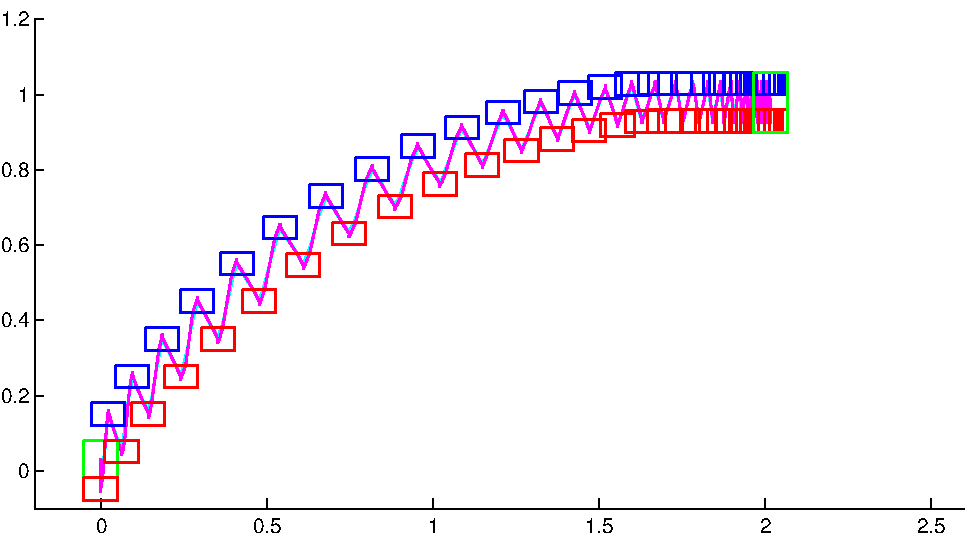
\includegraphics[scale=.46]{figures/steps1.pdf}
 \label{Fig:Results1a}
 }
 \subfigure[]{
 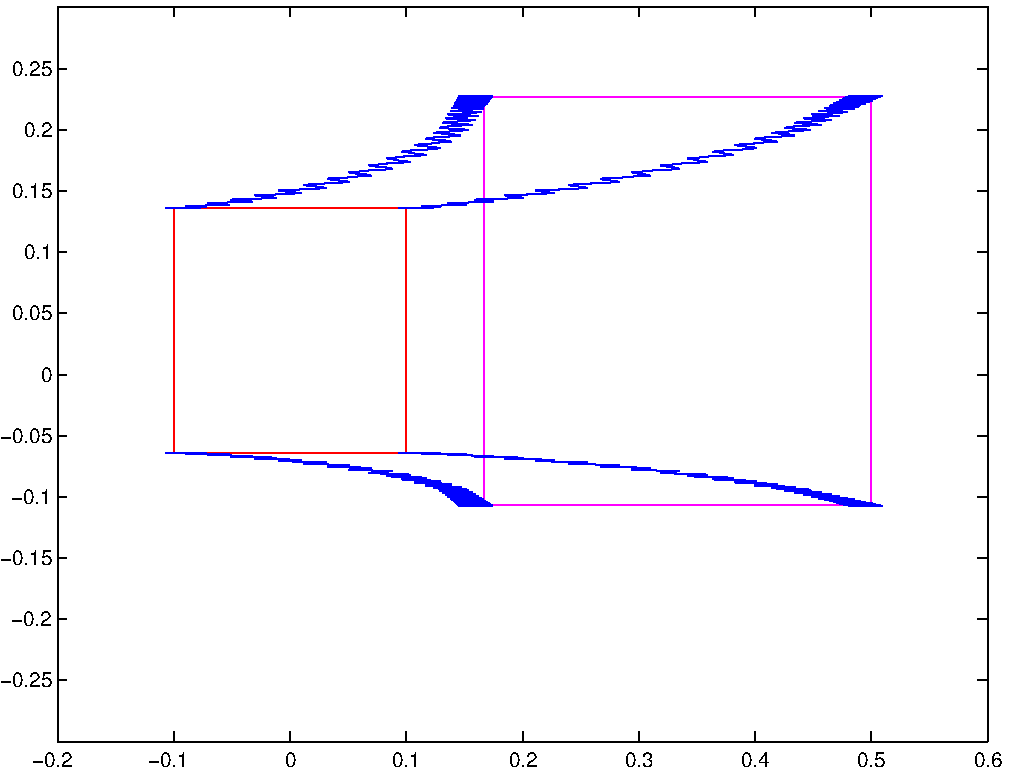
\includegraphics[scale=.27]{figures/features1.pdf}
 \label{Fig:Results1b}
 }
 \subfigure[]{
 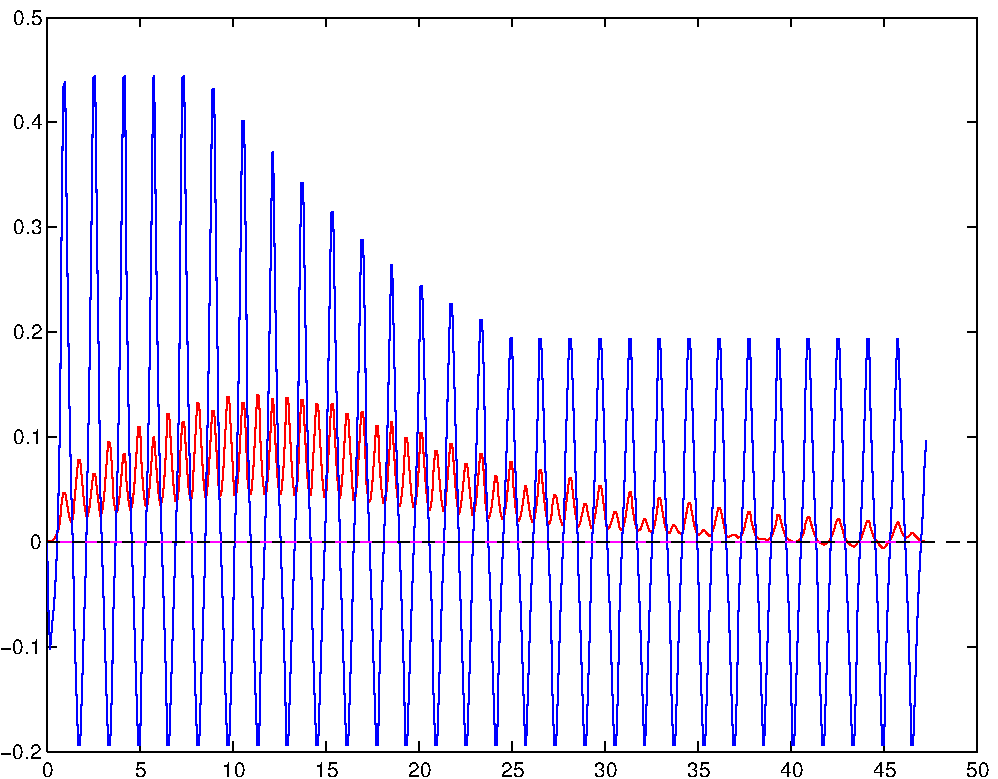
\includegraphics[scale=.27]{figures/velocities1.pdf}
 \label{Fig:Results1c}
 }
 \caption[]{\label{Fig:Results1}\small{In~\ref{Fig:Results1a}, we show the trajectory of the robot in the $x,y$ plane. The initial and final double stance phases appear in green. The single stance support feet appear in red (resp. blue) for the right (resp. left) foot. In pink, we depicted the CoP trajectory, which can be observed to remain safely in the support polygon, and in light blue the CoM trajectory. In \ref{Fig:Results1b}, we depict (in blue) the trajectory of the features in the image, with the initial positions in red and the desired positions in pink, for the first simulation.  Finally, the evolution of the velocities is shown in \ref{Fig:Results1c}. It is interesting to note the offset of the oscillatory velocity in $x$ and $y$ due to the features errors.}}
 \end{figure*}


\begin{figure*}[ht]
 \centering
  \subfigure[]{
 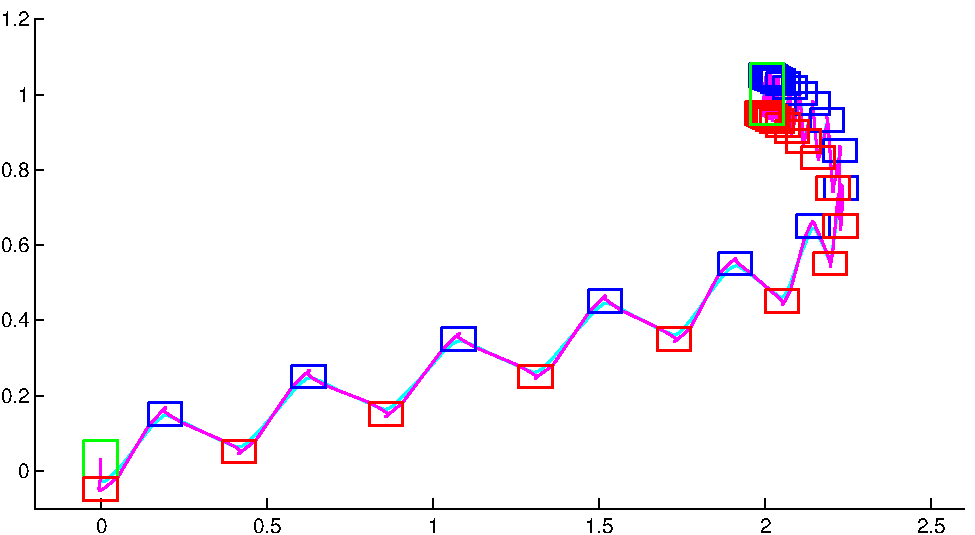
\includegraphics[scale=.46]{figures/steps2.pdf}
 \label{Fig:Results2b}
 }
 \subfigure[]{
 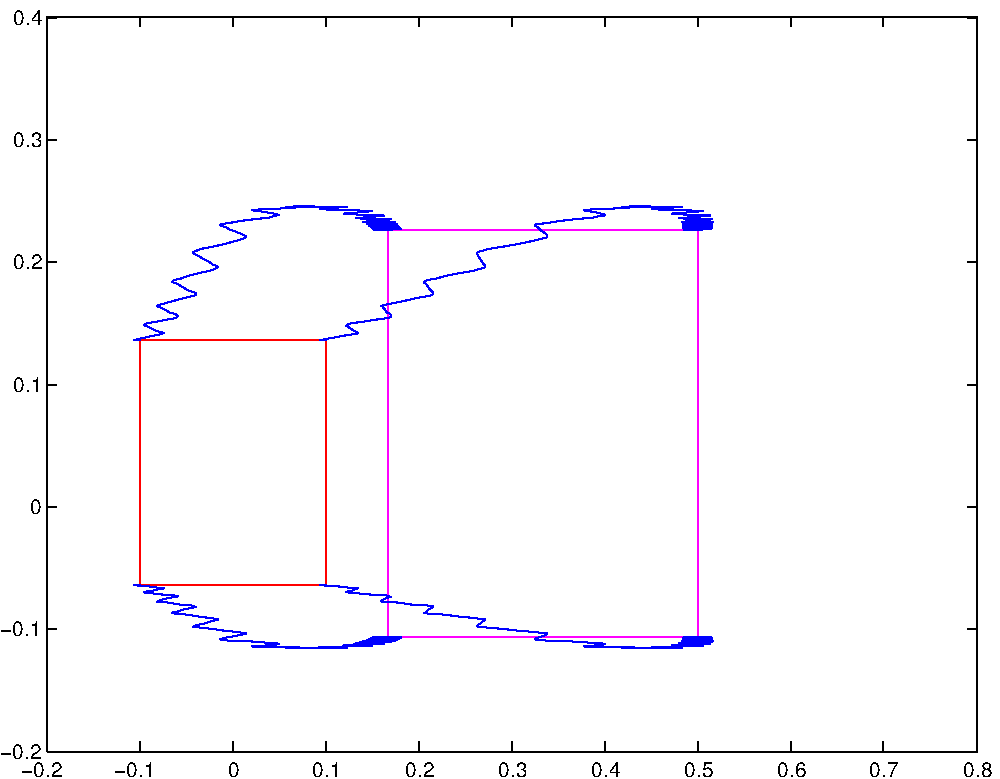
\includegraphics[scale=.27]{figures/features2.pdf}
 \label{Fig:Results2a}
 }
 \subfigure[]{
 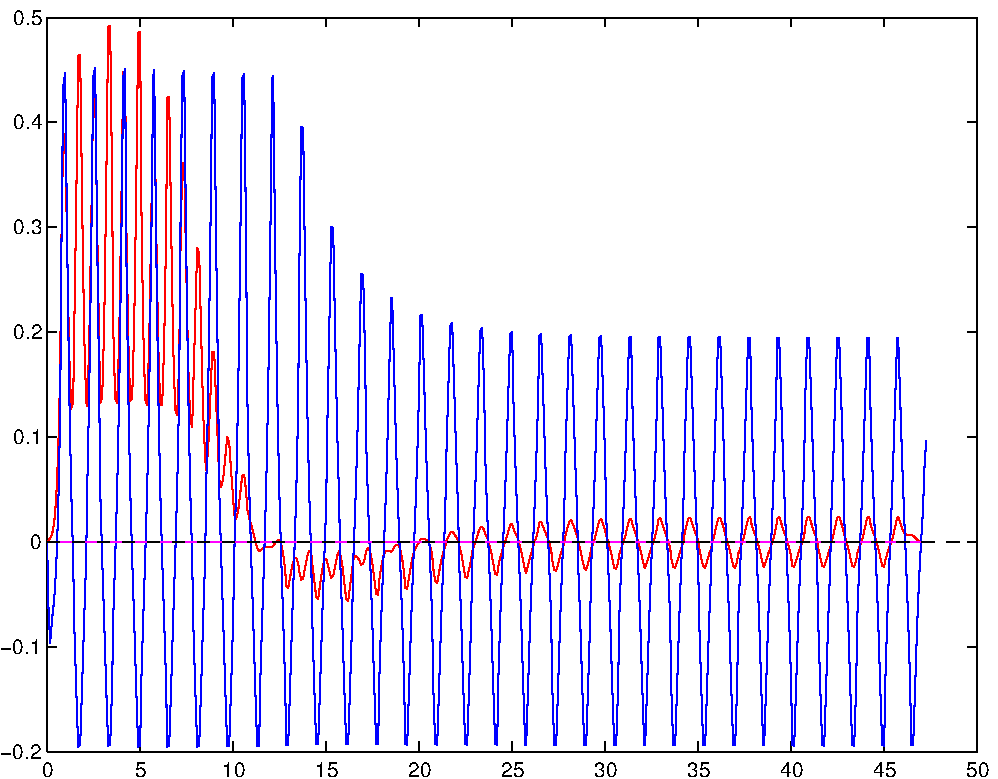
\includegraphics[scale=.27]{figures/velocities2.pdf}
 \label{Fig:Results2c}
 }
 
 \caption[]{\label{Fig:Results2}\small{The behavior of our system in the second simulation ($\beta$ is 10 times higher), with the same graphical conventions as in Fig.~\ref{Fig:Results1}. The robot is following a quite distinct trajectory, with a backwards part close to the end. As the priority is to minimize features errors, disregarding the jerks, high velocities are taken.}}
 \end{figure*}

Now we evaluate the trajectory with rotation. We recall that the rotation velocity control is decoupled from the $x$ and $y$ velocities control. It works as follows: The rotation velocity controller sets (in a decoupled way) the angular position while the main controller (QP) adapts the $x,y$ velocities in terms of this given angular position (which is known in the horizon), the visual errors, footsteps centering and jerks minimization. The results of a first simulation involving rotation is shown in Fig.~\ref{Fig:Results3}. One can observe that the dynamical balance is kept, and that most of the correction related to the rotation is done at the beginning of the trajectory. Also, in Fig.~\ref{Fig:Results4}, we can see that it is robust to perturbations: The same trajectory is followed as in Fig.~\ref{Fig:Results3} but a strong perturbation in the CoM position has been introduced, inducing peaks in the cost function and in the velocities. However, the perturbation is recovered quasi-instantly.

%  \begin{figure}[h]
%  \centering
%  \includegraphics[scale=.25]{featuresA1.png}
%  \caption[]{ \label{Fig:Image} Left image of the stereo pair.}
%  \end{figure}

\begin{figure*}[ht]
 \centering
  \subfigure[]{
 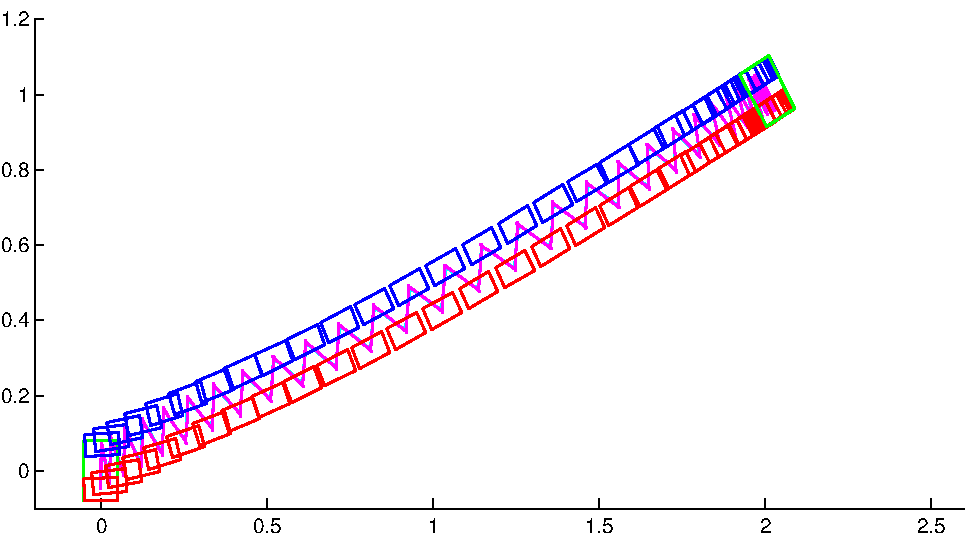
\includegraphics[scale=.46]{figures/steps3.pdf}
 \label{Fig:Results3b}
 }
 \subfigure[]{
 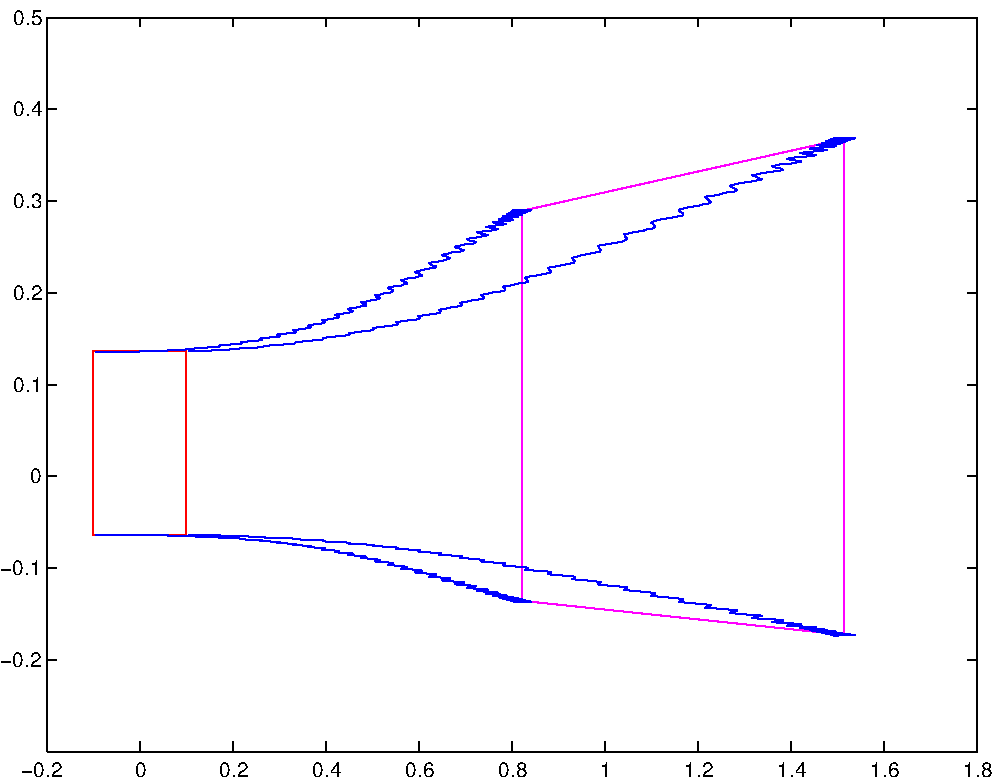
\includegraphics[scale=.27]{figures/features3.pdf}
 \label{Fig:Results3a}
 }
 \subfigure[]{
 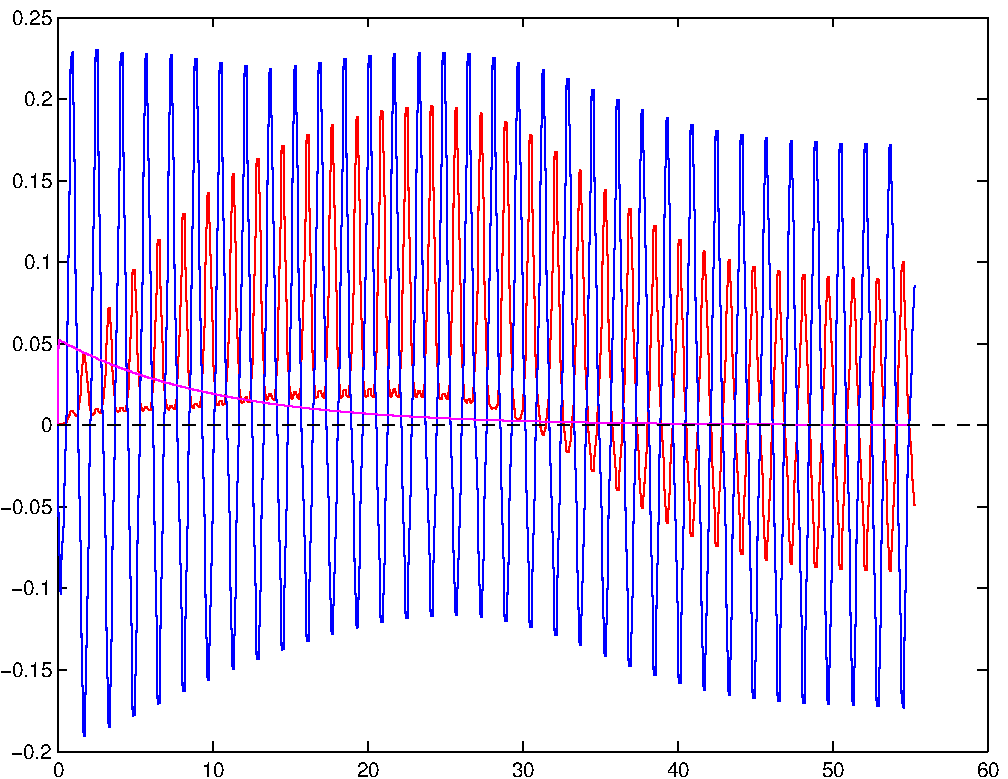
\includegraphics[scale=.27]{figures/velocities3.pdf}
 \label{Fig:Results3c}
 }
 \caption[]{\label{Fig:Results3}\small{The behavior of our system in the third simulation, involving rotation, with the same graphical conventions as in Fig.~\ref{Fig:Results1}. The robot is walking in the sagittal direction most of the time, after an initial rotation. The amplitude of the oscillation of the CoM and subsequently of the features are smaller than in the first simulation. However, we can see a non-negligible component of velocity in the positive $y$ direction, since the angle is not fully compensated. When the angle is almost fully compensated, this component disappears.}}
 \end{figure*}

\begin{figure*}[ht]
 \centering
 \subfigure[]{
 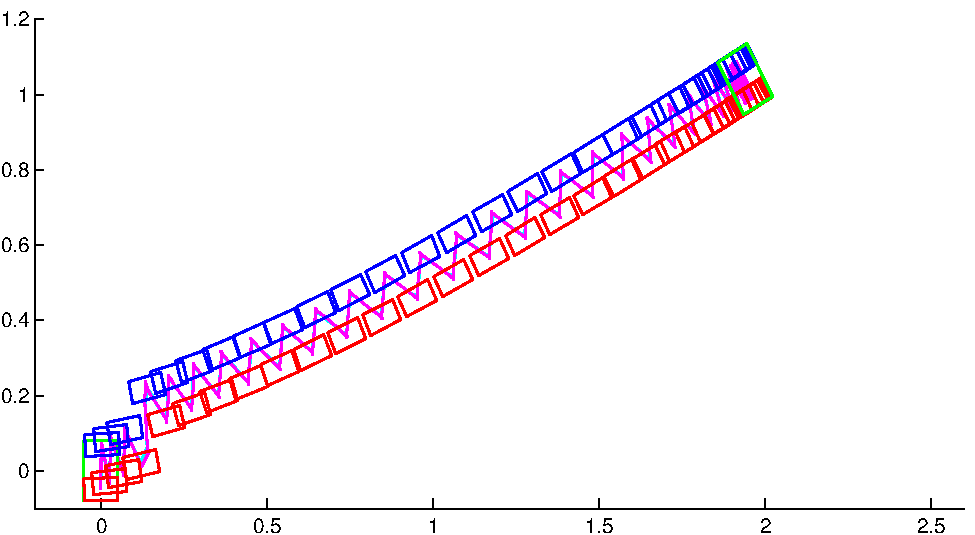
\includegraphics[scale=.46]{figures/steps4.pdf}
 \label{Fig:Results4a}
 }
  \subfigure[]{
 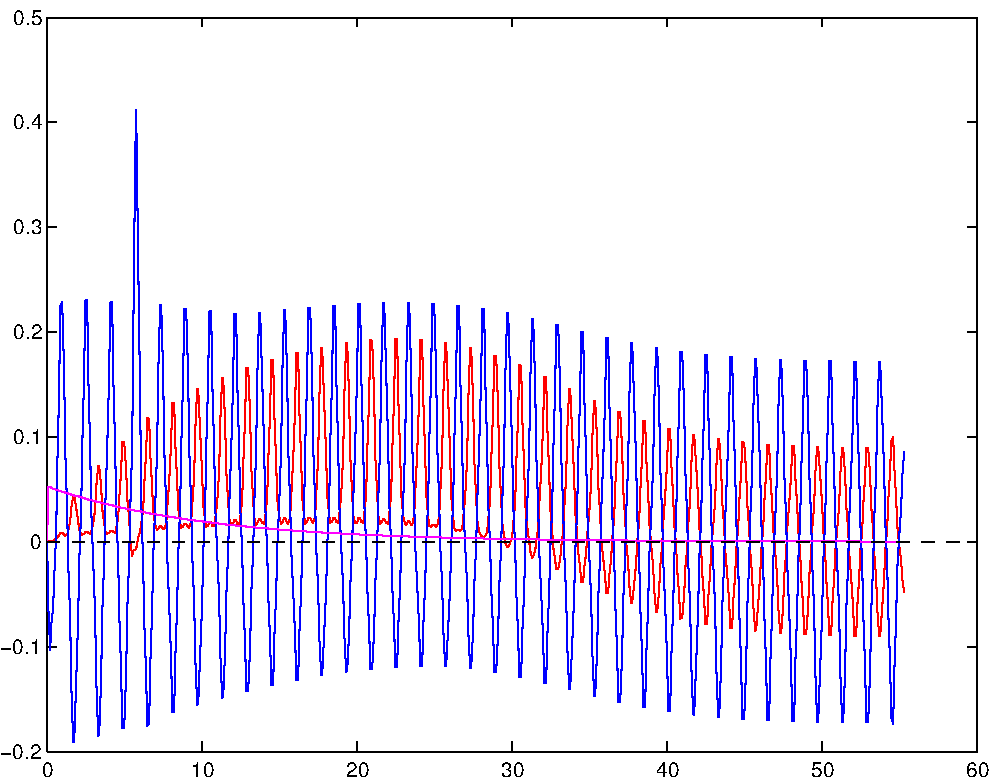
\includegraphics[scale=.27]{figures/velocities4.pdf}
 \label{Fig:Results4b}
 }
 \subfigure[]{
 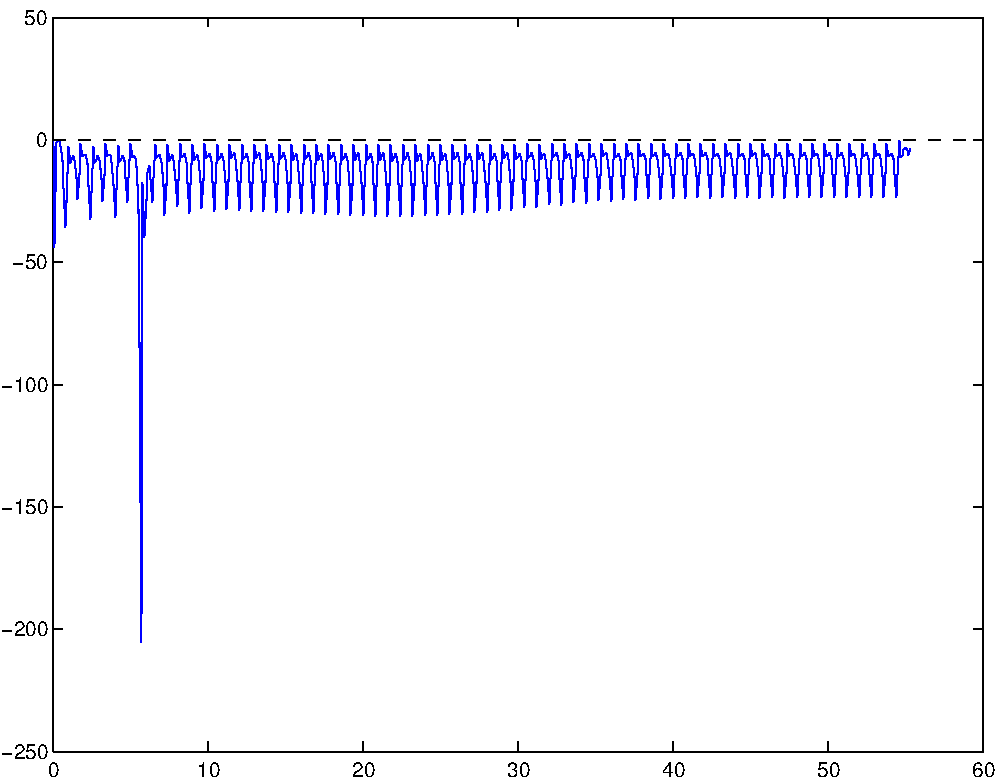
\includegraphics[scale=.27]{figures/objective4.pdf}
 \label{Fig:Results4c}
 }
 \caption[]{\label{Fig:Results4}\small{The behavior of our system in the fourth simulation, with the same graphical conventions as in Fig.~\ref{Fig:Results1}. The robot is following a trajectory similar to the one of Fig.~\ref{Fig:Results3}. After a few footsteps, a strong perturbation is applied to the CoM, inducing a peak in the velocities graph (Fig.~\ref{Fig:Results4b}) and in the cost function value (Fig.~\ref{Fig:Results4c}). The perturbation is quasi-instantly recovered.}}
 \end{figure*}

We have already explained how a local linearization is made to maintain the QP formulation. The performance of this linearization depends of the distance traveled inside the horizon, which depends on the velocity of the robot and the size of the horizon. In Fig.~\ref{Fig:Results5}, we can see the linearized and real features trajectories for a given CoM trajectory. As expected, close to the beginning (the linearization point) the trajectories are quite similar, while the final positions differ much more. This is an extreme situation, since usual metric displacements in the horizon are much smaller than this one. In any case, horizon displacements are bigger when the visual errors are bigger (the robot is far from the desired position) in which case the robot just needs a tendency. But when the errors are getting smaller, the robot needs more precision. In this case, displacements in the horizon becomes smaller so that the difference between the real model and the linearized one becomes negligible.

\begin{figure}[ht]
 \centering
 %\subfigure[]{
 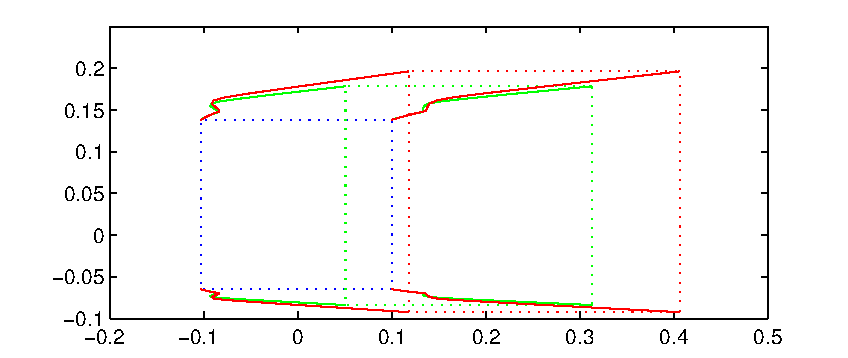
\includegraphics[scale=.6]{figures/comparison_linearization.pdf}
 %\label{Fig:Results2a}
 %}
 % \subfigure[]{
 %\includegraphics[scale=.6]{comparison_linearization_com.pdf}
 %\label{Fig:Results2b}
 %}
 \caption{\label{Fig:Results5}\small{In this figure, we show the trajectory of the visual features in one iteration of the QP, and compare the evolution of the features obtained by the linearization model (green lines) and features obtained by the non-linear model (red lines).}}
 \end{figure}

Due to the walking nature, we have oscillations in the features trajectories. If we use instantaneous errors measurements, the system will never converge, due to these oscillations. One of the main advantages of using MPC is that it naturally filters these oscillations. It is remarkable that, in comparison with~\cite{DuneIROS2010}, we do not need to model explicitly the sway motion of the robot and the resulting motion of the visual features. The system could oscillate inside the horizon (and it does), but at the end, the optimal control is taken without oscillations (Fig.~\ref{Fig:Results6}).

\begin{figure}[ht]
 \centering
 \subfigure[]{
 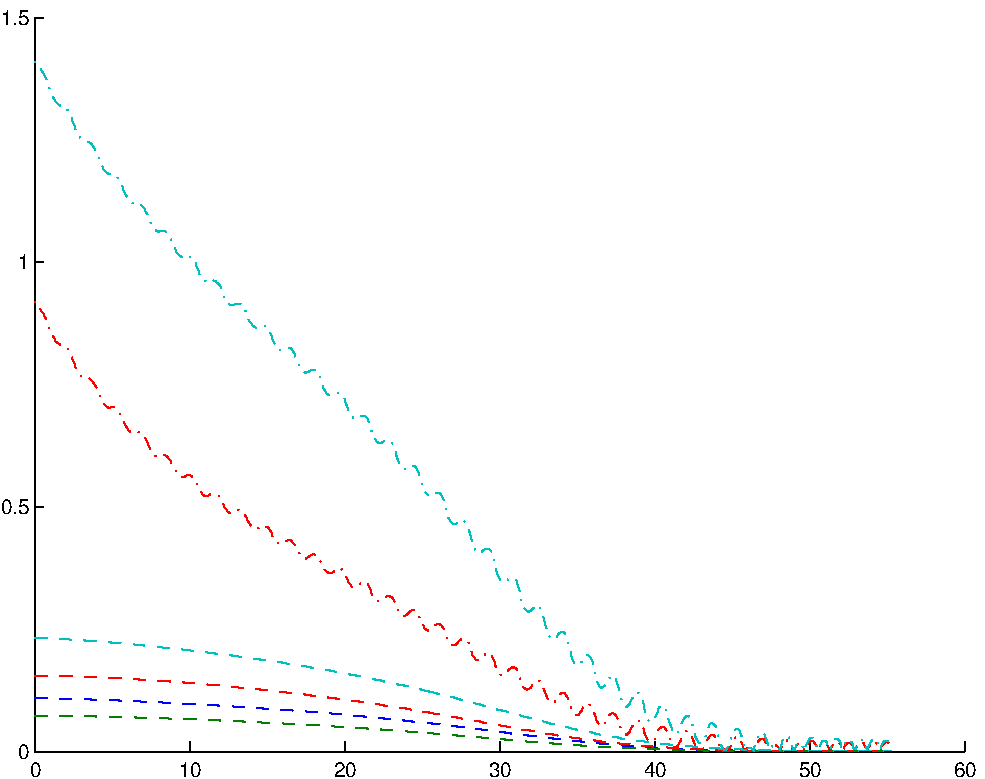
\includegraphics[scale=.23]{figures/instantaneus_errors.pdf}
 \label{Fig:Results6a}
 }
  \subfigure[]{
 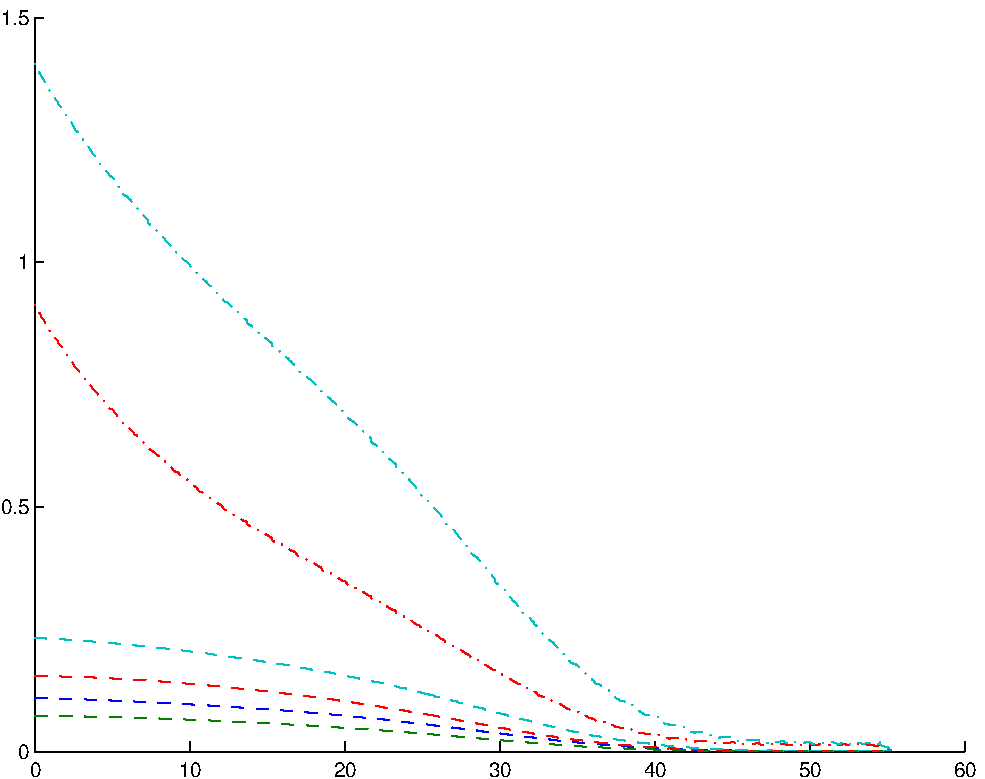
\includegraphics[scale=.23]{figures/horizon_errors.pdf}
 \label{Fig:Results6b}
 }
 \caption[]{\label{Fig:Results6}\small{Evolution of the errors for the $u,v$ components of each feature, in the second simulation. In \ref{Fig:Results6a}, we depict the instantaneous errors along time, and in \ref{Fig:Results6b}, we depict the errors estimated in the horizon (i.e. individual terms of Eq.~ \ref{Eq:MinVisualFeatures2}, normalized by the size of the horizon). Observe that the sway motion of the robot induces oscillations of the $v$ components in the instantaneous errors, and that these oscillations are not present in the errors estimated in the horizon window.}}
 \end{figure}

\section{Conclusion}
\label{sec:conclusions}
Since the original proposal for walking generation proposed in~\cite{Kajita2003}, most of the efforts in the literature have focused in dynamical balance and stability. In this paper, we have proposed a novel approach to close the control loop by introducing visual information into the walking pattern generation. Our online pattern generator integrates the regulation of the relative pose of 3D image features while simultaneous ensuring safety and stability. In order to keep the optimization formulation as a QP, the perspective projection equations have been linearized around the features positions at the beginning of each cycle. However, our current approach uses 3-D information that strongly depends on the localization. As a future work, we wish to drop the need of 3-D information by predicting the image positions of the landmarks in terms on the velocity of the robot in the horizon (IBVS); we also plan to perform real experiments on the HRP-2 humanoid platform.
